\section{Community Detection}
We considered two different approaches to identifying communities: spectral clustering and Louvain Method.
\begin{figure}[!htb]
  \centering
  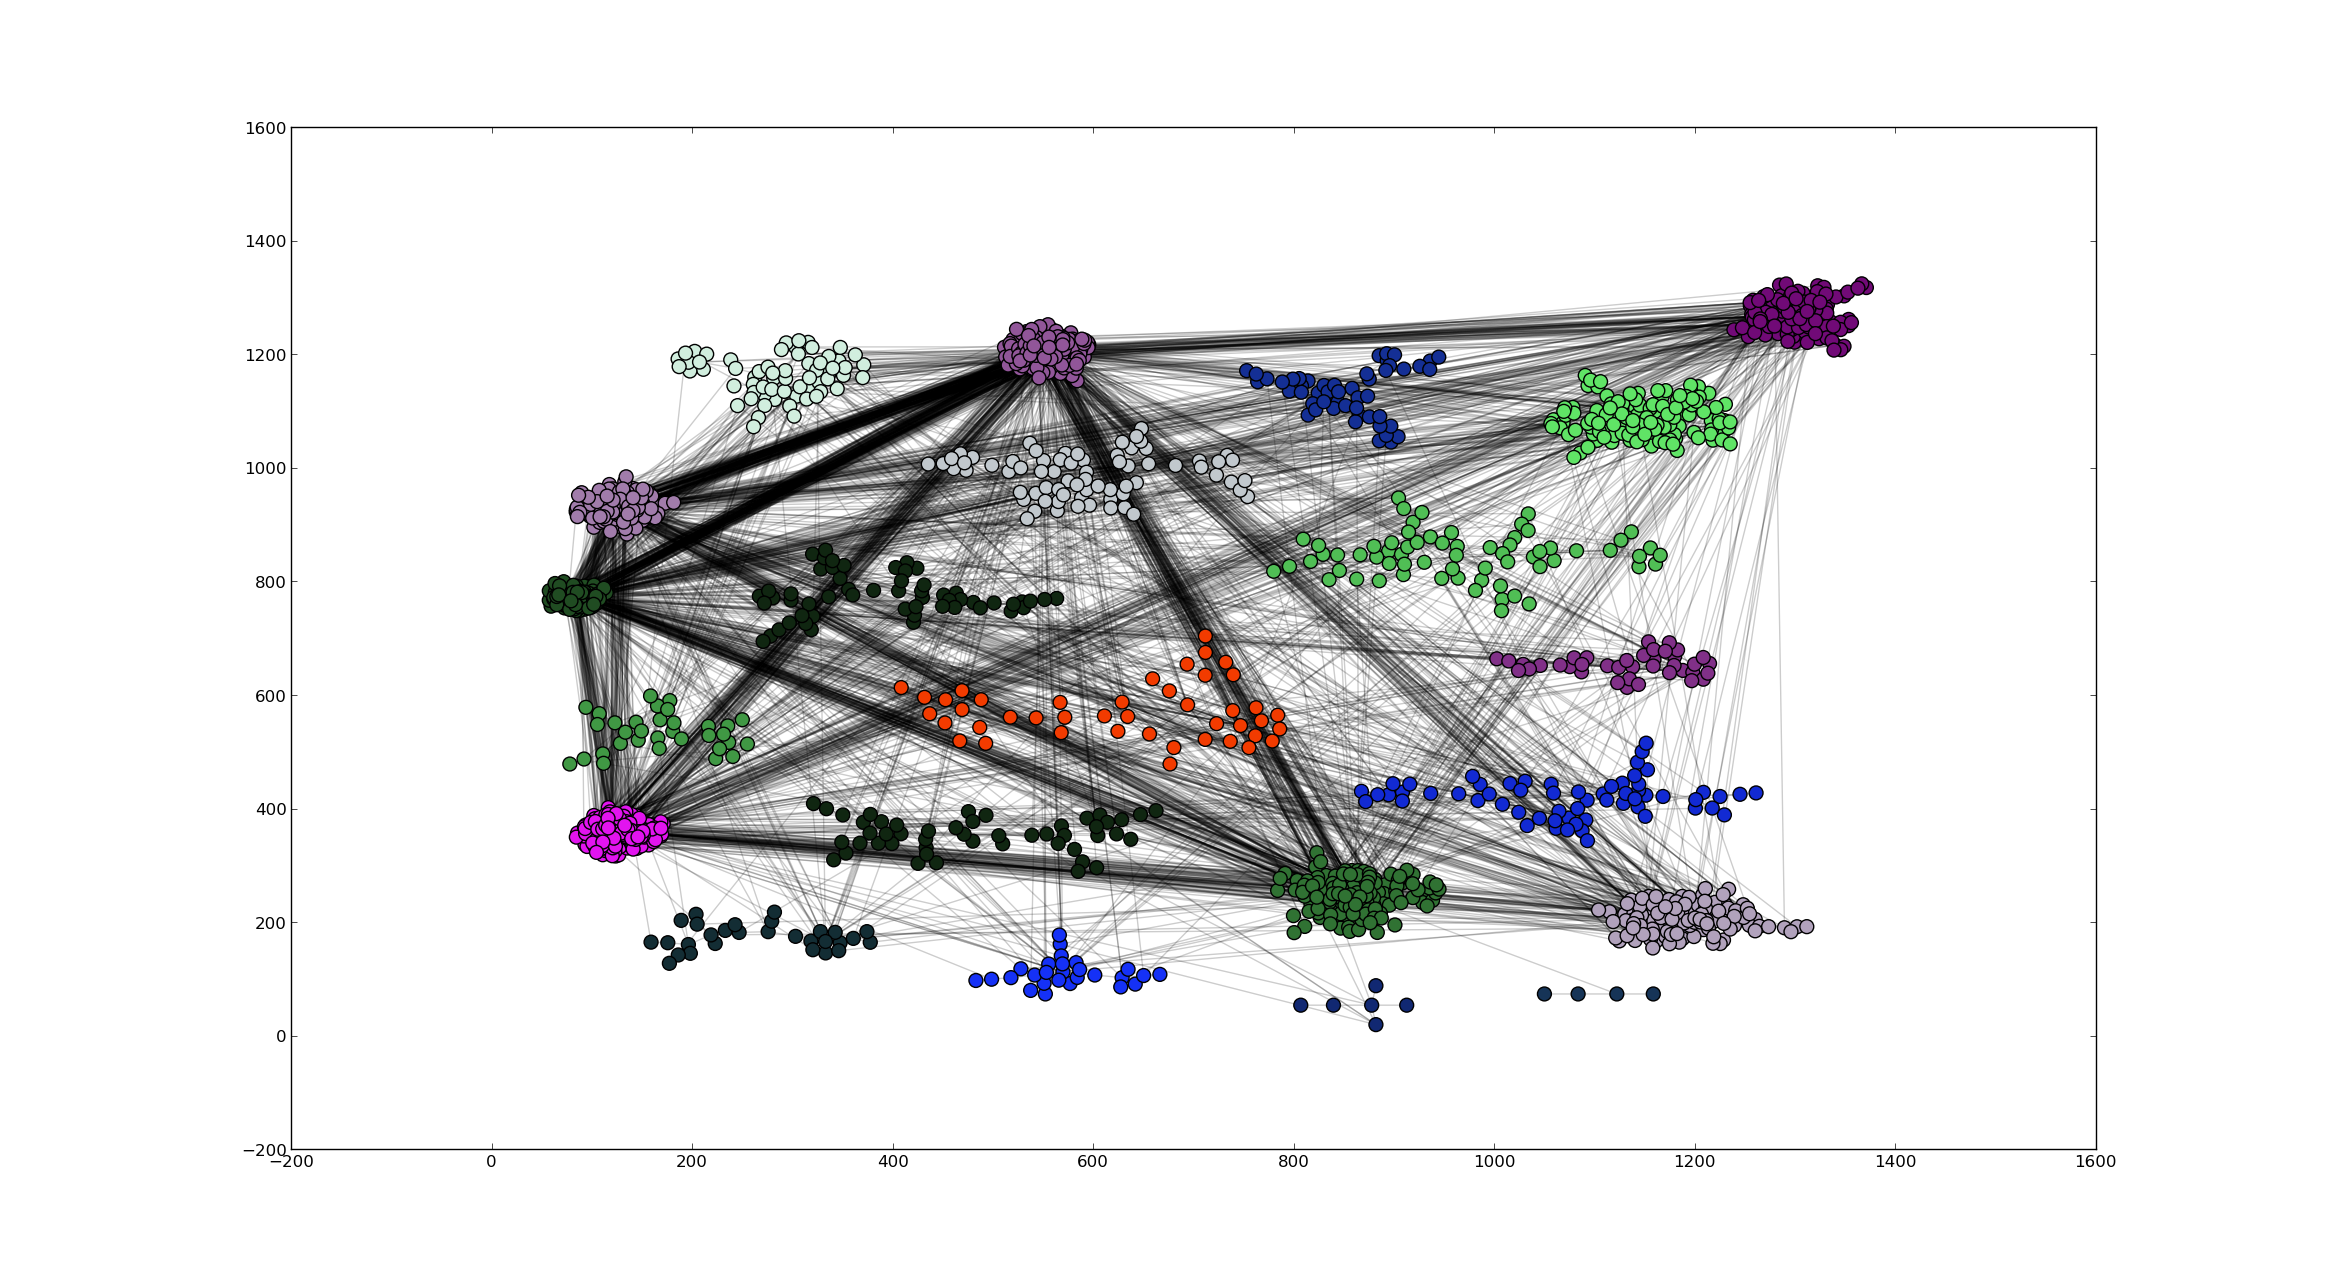
\includegraphics[width=.8\linewidth]{louvain_best.png}
  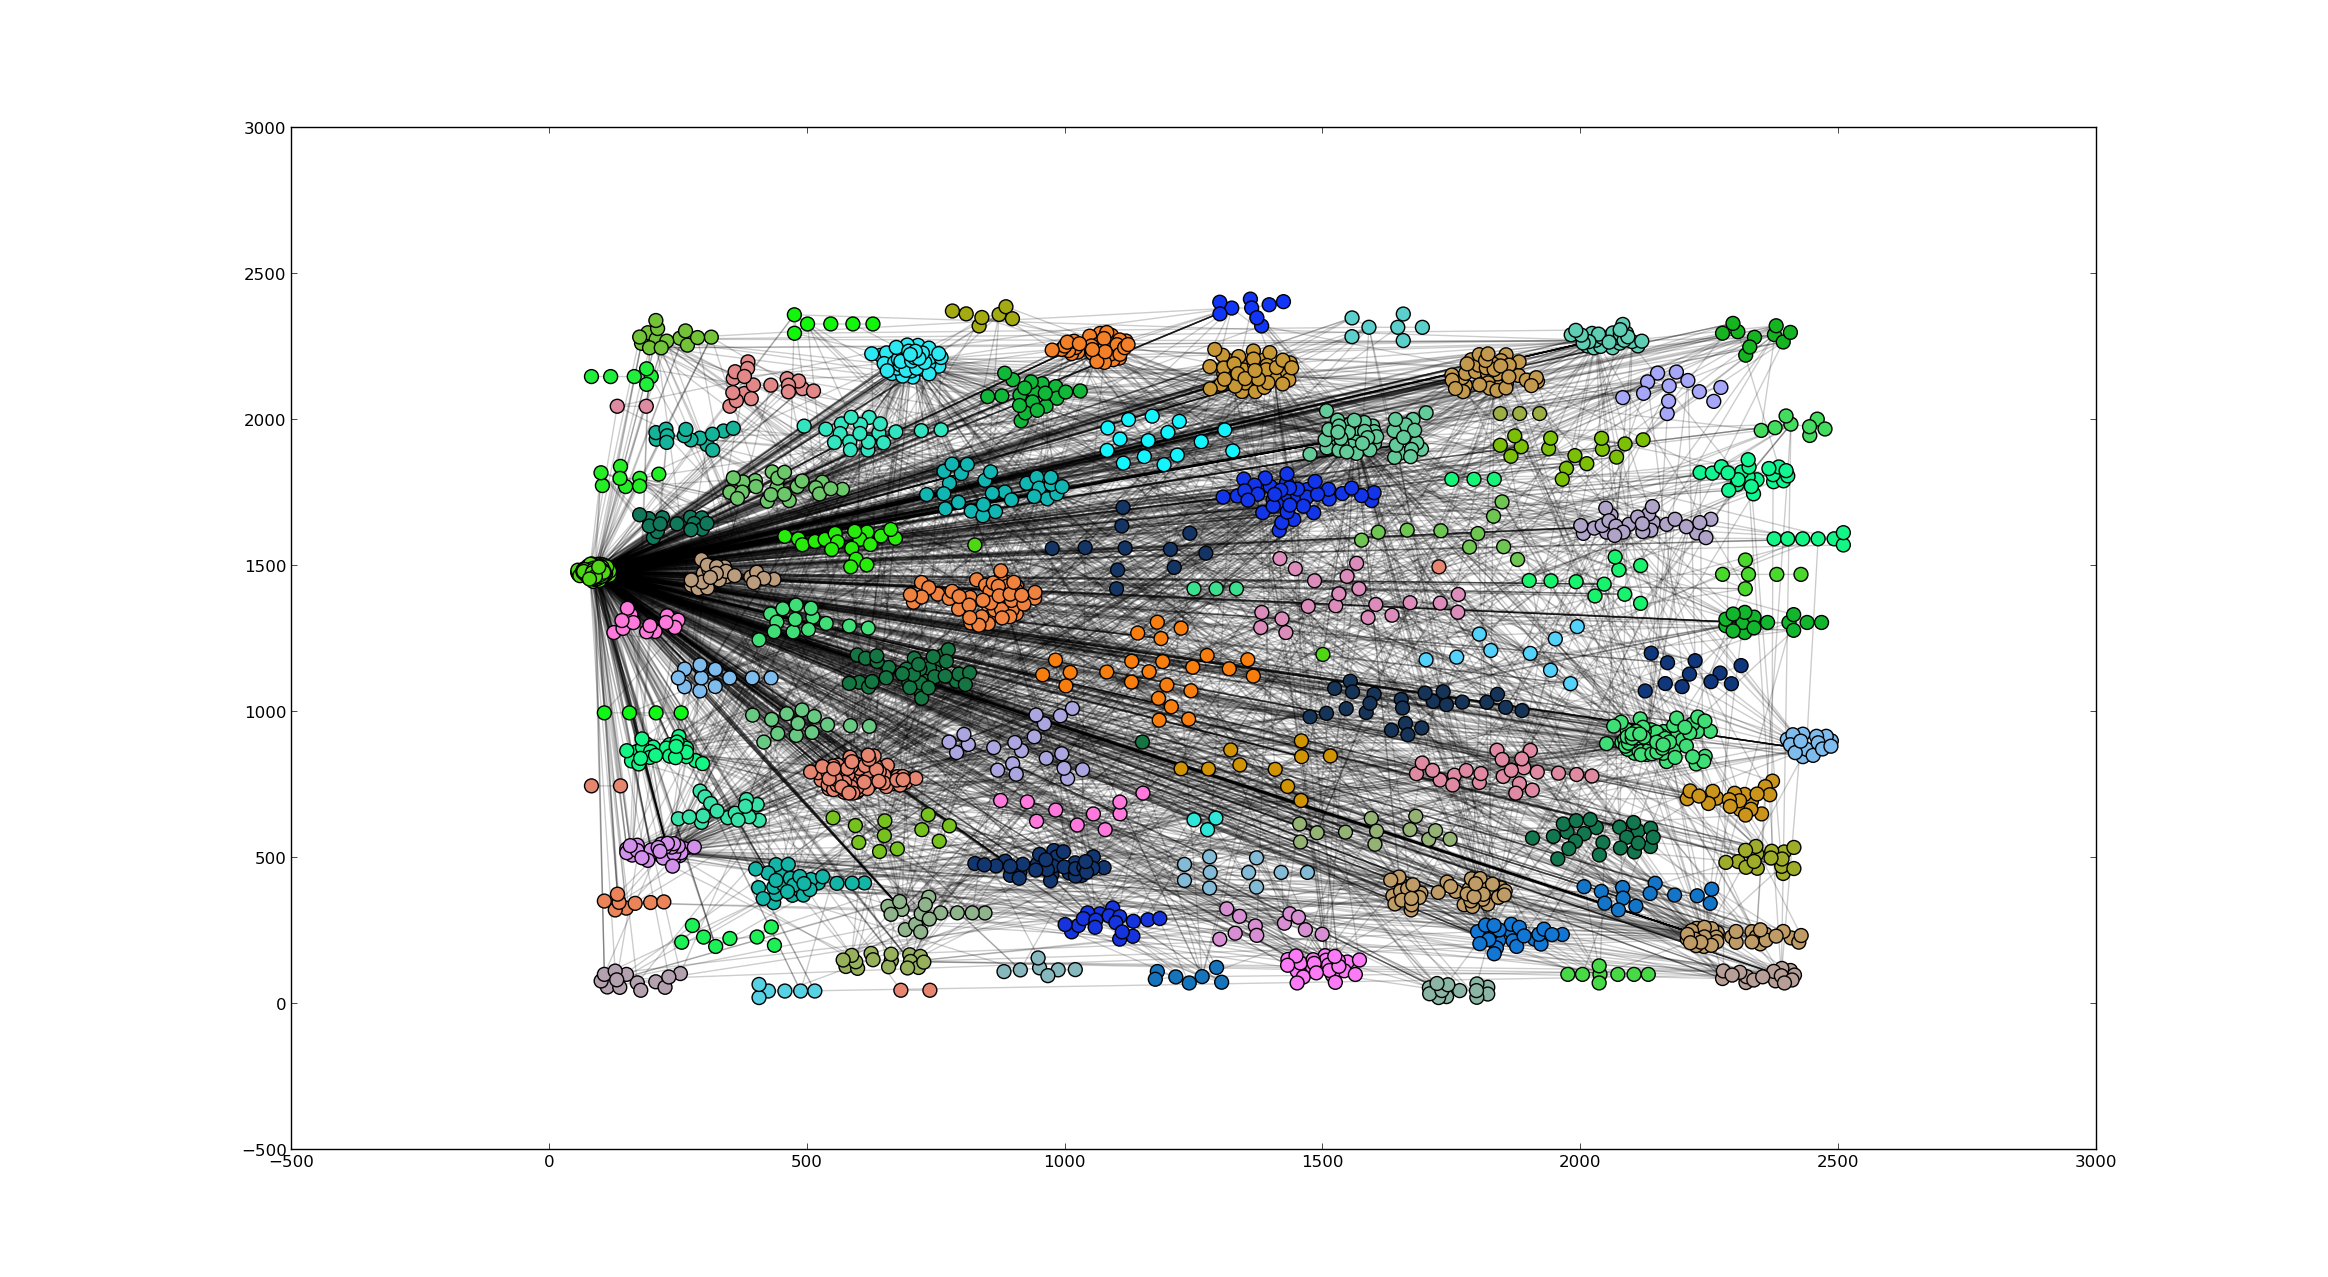
\includegraphics[width=.8\linewidth]{spectral_best.png}
  \caption{Visualization of the results of the highest modularity partitioning of 6.002x Fall 2012. On the top is the the best Louvain Method partition. On the bottom is the best spectral clustering partition.}
  \label{Louvain_best}
\end{figure}

\subsection{Spectral Clustering}

Spectral clustering is a group of techniques that transforms the initial set of verticies in space by using eigenvectors. After this transformation, the points are clustered using a standard algorithm\cite{2010PhR...486...75F}. Spectral clustering can be broken down into 3 parts

\begin{description}
  \item[Affinity Matrix] The algorithm uses an affinity matrix that describes the similarity between two vertices. In our case, the affinity matrix is exactly an instance of the Interaction Graph. This works because the $ij$ entry of an Interaction Graph encodes how the strength of the relationship between $i$ and $j$. 
  
  \item[Dimension Reduction] The algorithm uses the spectrum of the graph Laplacian to reduce the dimension of the matrix.  The Laplacian, L, of the graph is defined as 
  \begin{equation}
  L = D - A
  \end{equation}
  where $D$ is a diagonal matrix with $d_{ii} = deg[i]$ and $A$ is the adjacency matrix. In our implementation\footnote{In this paper, we use an implementation of spectral clustering and discrete clustering provided by scikit-learn\cite{spectral}.}, we use the normalized graph Laplacian which is defined as 
  \begin{equation}
  L' = D^{-\frac{1}{2}}LD^{-\frac{1}{2}}
  \end{equation}
  
  This is preferred to the unnormalized Laplacian because it performs better under general conditions \cite{von2008consistency}. Using the eigenvectors of the normalized Laplacian, each vertex is transformed into a lower dimension space where the coordinates are elements of the eigenvectors. This reduction is important because it makes the important features of the initial matrix more prominent before applying clustering. Thus, this method allows clusters to be identified that would not have been identified by standard clustering techniques. For example, spectral clustering tends to transform the initial into points into a convex sets of points, which are easier to cluster\cite{2010PhR...486...75F}.
  
  \item[Clustering] The algorithm uses a discrete method proposed by Yu and Shi to do clustering in the lower dimension space. This method was chosen over KMeans for clustering because it is often faster and more robust to random initialization than KMeans\cite{yu2003multiclass}. The clustering is found by iteratively searching for a discrete partition closest to the eigenvector embedding. This done by first normalizing the eigenvector embedding to the space of the partition matrix. Next, a we fix an optimal discrete partition matrix and then calculate the optimal rotation matrix. These to steps are performed until convergence. The discrete partition matrix is returned as the solution to the clustering problem. 
 
\end{description}

\subsection{Louvain Method}
The Louvain method is a greedy optimization method for determining communities in large networks \cite{2008JSMTE..10..008B}. It seeks to optimize the modularity of a partition of the network. Given a partition of the graph, the modularity measures the relative frequency of links inside communities as compared to links between communities. It is scalar value between -1 and 1 and is calculated as follows

\begin{equation}
Q = \frac{1}{2m} \sum_{i,k} \left[ A_{ij} - \frac{k_i k_j}{2m}\right]\delta(c_i,c_j)
\end{equation}

where $A_{ij}$ is the weight of the edge between $i$ and $j$, $k_i = \sum_{j}A_{ij}$, $c_i$ is the community that $i$ is assigned to, the $\delta(u,v)$ is 1 if $u=v$ and 0 otherwise, and $m = \frac{1}{2}\sum_{ij}A_{ij}$. 

Exact modularity optimization is NP-hard \cite{2008JSMTE..10..008B}. The algorithm starts by assigning a unique community to each node and then iteratively performing two steps until maximum modularity is achieved. First, the method looks at every node $i$ and its each of its neighbors $j$. Node $i$ is removed from its community and added to the community of $j$ where the gain in modularity is highest. If the modularity cannot be improved by moving $i$, then the community assignment will not change. This is repeated until no more changes in community can be performed to increase modularity. The second step is to build a new network where the nodes are the communities discovered in the first step. Edges between nodes in the same community are self loops in the is new graph. These steps are repeated iteratively until no more changes occur during an iteration, which means a maximum of modularity has been reached. This produces a hierarchy of communities. This method has been observed to be very fast and appears to run in $O(nlogn)$\cite{2008JSMTE..10..008B}, where $n$ is the number of nodes in the network\footnote{In this paper, we use an implementation for directed graphs for the NetworkX library \cite{louvain}.}.



